\documentclass[10pt,twoside,twocolumn,openany]{dndbook}
\let\chaptername\relax

\usepackage[spanish]{babel}
\usepackage[utf8]{inputenc}
\usepackage[singlelinecheck=false]{caption}
\usepackage{lipsum}
\usepackage{listings}
\usepackage{shortvrb}
\usepackage{stfloats}
\usepackage{ifoddpage}
\usepackage{graphicx}
\usepackage{tikz}
\usepackage{hyperref}

\hypersetup{
  colorlinks=true,
  linkcolor=red,
  pdfauthor={Moisés Serrano Samudio},
  pdftitle={La pintura maldita},
  pdfsubject={one-shot},
  pdfkeywords={Dungeon and Dragons, DnD, 5e, exploración}
}

\DndSetFonts[section-style = \linespread{.9} \color{titlered} \LARGE \scshape \RaggedRight]

\title{La pintura maldita\\
\large One shot para personajes de nivel 3}
\author{linkmoises}
\date{\today}

\begin{document}

%% Portada
\newpage
\thispagestyle{empty}
\mbox{}
\begin{figure}
  \begin{tikzpicture}[remember picture,overlay]
    \begin{scope}
    \node [xshift=0cm,yshift=0cm] at (current page.center){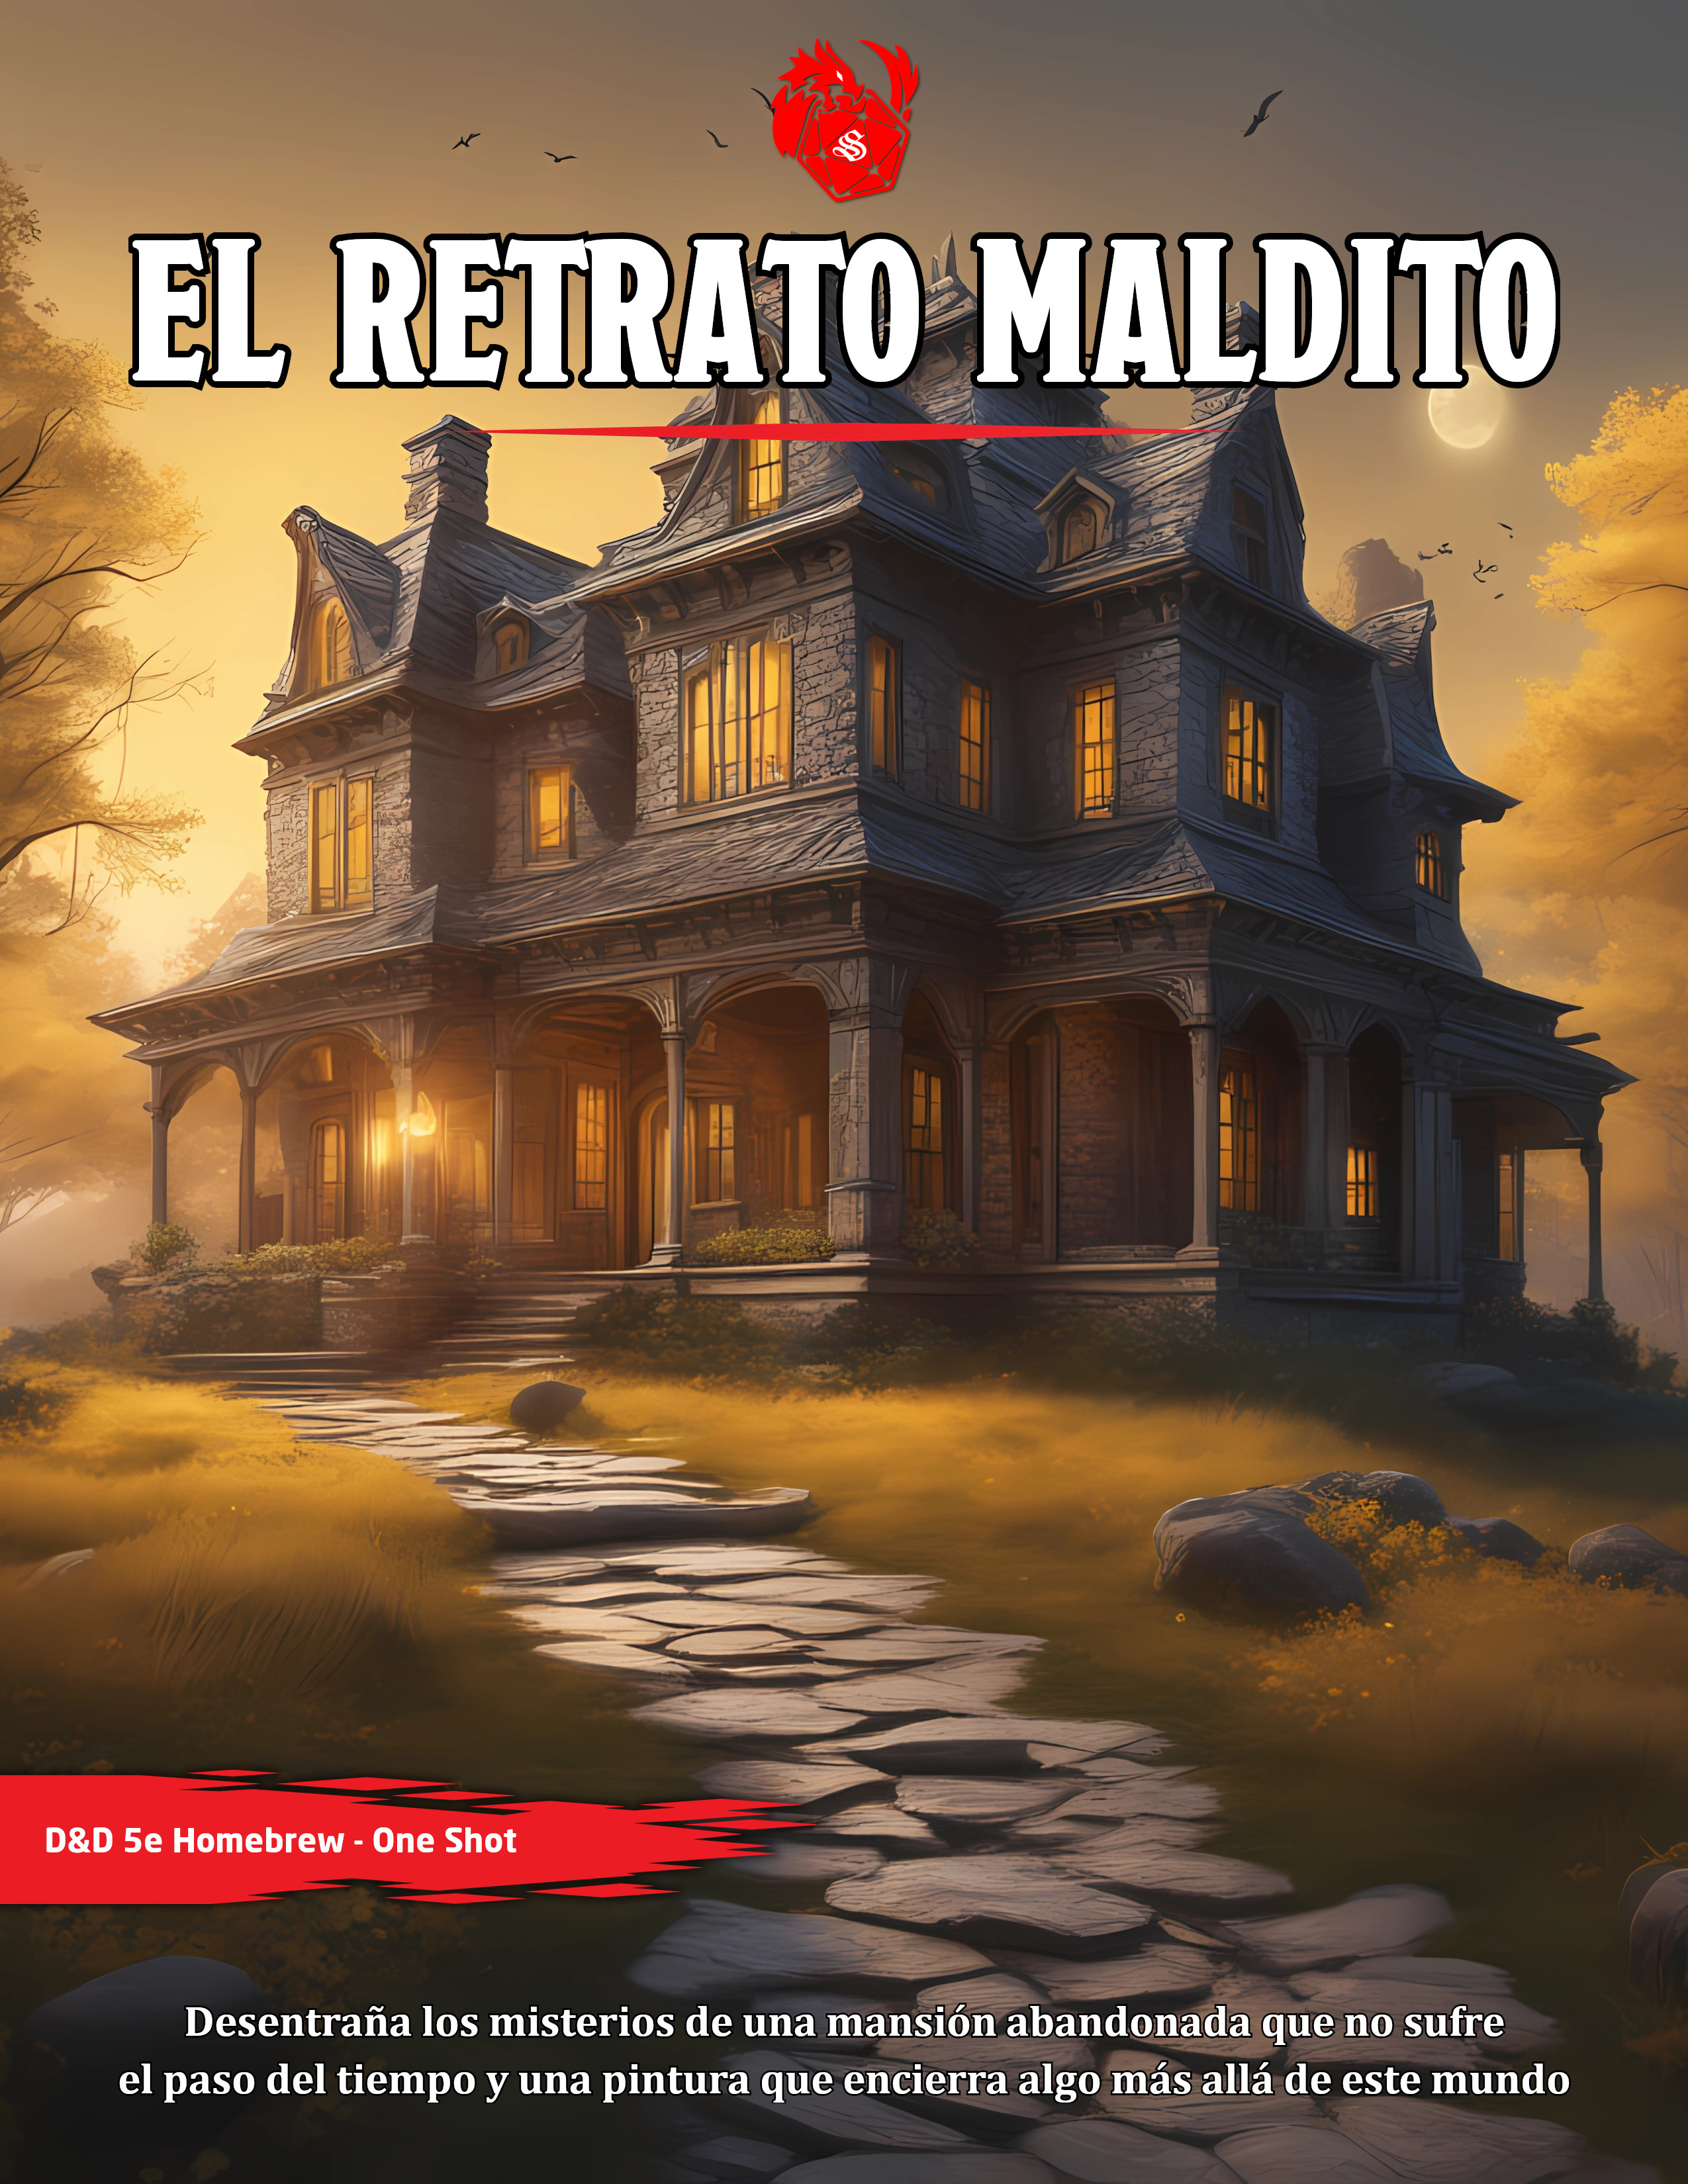
\includegraphics[width=\paperwidth]{covers/3-el-retrato-maldito.jpg}};
    \end{scope}
  \end{tikzpicture}
\end{figure}
%% Finaliza portada

\frontmatter

\maketitle

\mainmatter

\part*{El retrato maldito}

\chapter*{El retrato maldito}
\addcontentsline{toc}{chapter}{El retrato maldito}

\DndDropCapLine{E}{l sol se pone en el horizonte} teñiendo los cielos con tonos de naranja y 
púrpura, mientras te acercas a la ciudad de Neverwinter. La brisa fresca del mar se mezcla con 
el aroma de las flores silvestres que bordean el camino. Neverwinter, una ciudad de renombre en los
Reinos Olvidados, se extiende ante ti con sus calles bulliciosas y su animada vida nocturna.

En el corazón de esta metrópolis vibrante, las luces de las tabernas y los puestos de mercado 
comienzan a brillar, creando un espectáculo de colores y sonidos que invita a aventureros y 
comerciantes por igual. Sin embargo, esta noche, tu atención se centra en un enigma mucho más 
antiguo y oscuro: Villa Argentum.

\begin{DndReadAloud}
Situada en las afueras de Neverwinter, en una zona aislada y rodeada por un denso bosque ancestral,
Villa Argentum se yergue como un testigo silencioso del pasado. La mansión, de dos niveles, un 
ático y un sótano misterioso, se alza imponente y enigmática en medio del paisaje natural. Sus 
muros de piedra gris se erigen como guardianes antiguos, y sus ventanas altas han sido cubiertas
con tablones de madera, parecen ocultar secretos que la ciudad nunca ha conocido.

A medida que te acercas a Villa Argentum, sus torretas y picos de techos puntiagudos se recortan 
contra el cielo crepuscular, creando una imagen digna de un cuento de hadas sombrío. Los jardines 
que rodean la mansión están cubiertos por una maraña de rosales silvestres y setos descuidados, 
otorgándole una belleza marchita y encantadora.
\end{DndReadAloud}

\section{Presentación y gancho de aventura}

Villa Argentum lleva muchos, muchos años abandonada. Sirius Belmont, la última persona que vivió 
allí, se fue de la ciudad hace 100 años, sin que nadie recuerde aparentemente el motivo. Durante 
las últimas décadas, la casa ha permanecido abandonada y ha sido fruto de todo tipo de rumores y 
especulaciones.

Ha habido varios intentos de volverla a habitar, pero todos aquellos que se mudaron allí, acabaron
por marcharse al poco tiempo, argumentando que algo raro pasaba entre sus muros. Con el paso del 
tiempo, la propiedad dejó de provocar interés... hasta ahora.

La leyenda de Villa Argentum habla de un linaje olvidado y un pacto oscuro, y es ahora, en este
atardecer inquietante, que te has encontrado con la oportunidad de descubrir la verdad que se 
esconde tras sus puertas.

Los aventureros son ya héroes que empiezan a tener algo de fama. Dependiendo de la conformación 
del grupo o del tiempo de disponible, diversos ganchos de aventura pueden ser utilizados.

Los personajes reciben un mensaje de un viejo amigo o aliado que dice haber conocido a un 
descendiente de los dueños de Villa Argentum. El mensaje les informa que esta persona esta 
dispuesta a pagar una importante suma de piezas de oro ruega que acudan a la mansión a investigar
y disipar los rumores que se escuchan sobre Villa Argentum.

Otro gancho que puede ser utilizado sería que los personajes se enteran de que Villa Argentum está 
a la venta y se sienten atraídos por la oportunidad de adquirir una propiedad legendaria. Cuando 
llegan, se encuentran con una persona que se presenta como descendiente de los dueños de la 
mansión que se había criado muy lejos de aquel lugar y que recibía la noticia que la heredaba,
pero no esta interesado en vivir en ella por lo que desea venderla, pero también dilucidar los
rumores que existen sobre Villa Argentum.


\section{Sirius: Un descendiente carismático}

\begin{figure}
  \centering
  
\includegraphics[width=0.9\columnwidth]{media/sirius-belmont.png}
  \caption{Lord Sirius Belmont}
\end{figure}

Al llegar a Villa Argentum, se encuentran con una persona que habla con dos guardias, al notar 
la presencia del grupo, se despide de los guardias de manera amable y les da órdenes de custodiar 
el área de su propiedad familiar.

\begin{DndReadAloud}
  Sirius Belmont IV es un hombre joven, de poco más de treinta años, con facciones occidentales, 
  pero de piel bronceada. Viste de forma lujosa, haciendo ostentación de varios anillos, 
  pulseras y medallones, pero lo hace con total naturalidad. Es increíblemente atractivo y 
  tiene una personalidad magnética y atrayente. Siempre es encantador, elogia a sus 
  interlocutores y los hace sentirse tremendamente cómodos en su presencia. También es un 
  seductor nato, pero sólo con aquellos sujetos que él encuentra atractivos.
\end{DndReadAloud}

Sirius se interesará por el pasado de los personajes, por sus aventuras y se mostrará atento y 
encantador con ellos. También se fijará especialmente en todos aquellos que tengan un Carisma 
de 16 o superior, ya que los encontrará hermosos y atractivos. Les contará a los jugadores su 
pasado y la historia de su familia, aunque no comentará los motivos por los que su antepasado 
se marchó de la ciudad y dirá que no los conoce, que eso nunca se mencionaba en su casa, 
únicamente que algún día volverían a Neverwinter a reclamar lo que era suyo.

A pesar de su edad, es un hombre que ha viajado mucho y ha estado en multitud de lugares y conoce 
muchas historias sobre la exhuberancia de Luskan, el lejano desiero de Anauroch, 
la remota Longsaddle y su enigmática magocracia... incluso del Underdark y de las extrañas 
civilizaciones que existen en ella. Hablará de la belleza de esos lugares y también de los 
placeres que se pueden encontrar en ellos: comida, bebida, música, compañía carnal... 

\begin{DndComment}{¿Miente?}
  Durante toda la conversación, los jugadores podrán intentar hacer una prueba de Perspicacia CD 20. 
  Si la superan, sabrán que Sirius no está contando toda la verdad sobre su pasado. A la pregunta
  que hagan los jugadores, Sirius responderá con este contexto

\begin{itemize}
  \item Todas las historias que cuenta son reales
  \item Se avergüenza del pasado de su apellido
  \item Pretende comenzar una nueva vida en Neverwinter
\end{itemize}
\end{DndComment}

Sirius está mintiendo en todo momento, sólo que para descubrirle esta vez la prueba de perspicacia es de 
CD 22. Si es descubierto de nuevo, Sirius contará esta historia:

\begin{DndReadAloud}
Su tatarabuelo, Lord Sirius Belmont I forjó su riqueza y construyó Villa Argentum hace décadas atrás.
Era un joven noble de Neverwinter que amaba las fiestas y el arte. Un día conoció a su tataraabuela
Lady Evangeline Vanthorn, con quien se hizo amigo y luego amante. Ella era una extraordinaria 
pintora, pero un día ocurrió algo terrible que sus padres jamás le contaron que fue pero los obligo
a huir de Villa Argentum y retirarse al exilio. Volvió a Neverwinter con la esperanza de encontrar
respuestas a las preguntas de su pasado y reclamar su herencia que por derecho le corresponde, ya
que la casa, a pesar del tiempo está en un magnífico estado.
\end{DndReadAloud}

La realidad es que Sirius Belmont IV es, en realidad, el mismo que abandonó Neverwinter hace tantas 
décadas. A pesar de ser humano, su aspecto no ha envejecido un solo día, ya que un poderoso conjuro, 
una maldición, pende sobre él. Cuando era un joven noble de Neverwinter se dio al lujo y al 
hedonismo, disfrutando de sus riquezas y de su amor por el arte y las fiestas. Fue así como conoció
a Lady Evangeline Vanthorn, una joven noble de Waterdeep, de rango bajo, pero que era una 
extraordinaria pintora. Se hicieron amigos y, después, amantes. Evangeline dibujó un cuadro de 
Sirius que lo cautivó inmediatamente, ya que capturaba perfectamente su belleza, fortaleza y 
juventud. Se obsesionó con el retrato y con la idea de no envejecer nunca para disfrutar 
eternamente de una vida disoluta.

\begin{figure}
  \centering
  
\includegraphics[width=0.9\columnwidth]{media/evangeline-vanthorn.png}
  \caption{Lady Evangeline Vanthorn}
\end{figure}


\section{Créditos}

Las ilustraciones en este one shot, son creaciones de sus respectivos autores. Los mapas han sido 
creados con la herramienta \href{https://inkarnate.com/}{Inkarnate}. Estos son los enlaces a las 
ilustraciones originales:

\begin{itemize}
  \item A day in Hell por \href{https://licensing.pixels.com/featured/a-day-in-hell-jackson-parrish.html}{Jackson Parrish}.
\end{itemize}


\end{document}
